

\begin{center}
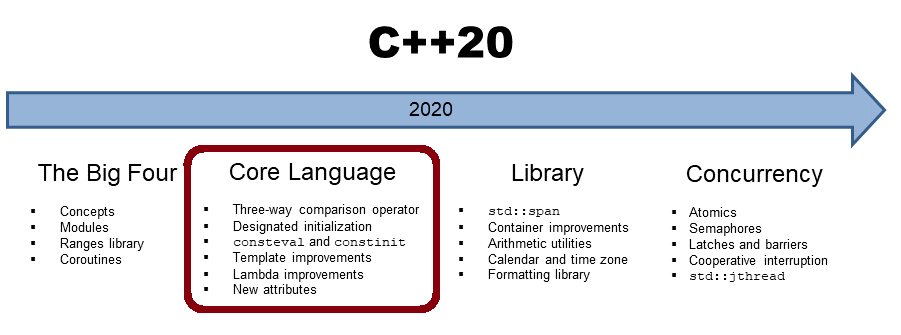
\includegraphics[width=1.0\textwidth]{content/2/chapter3/images/4.png}\\
\end{center}

\subsubsubsection{3.2.1\hspace{0.2cm}Three-Way Comparison Operator}

The three-way comparison operator <=>, or spaceship operator, determines, for two values A and B, whether A < B, A == B, or A > B.

By declaring the three-way comparison operator default, the compiler will attempt to generate a consistent relational operator for the class. In this case, you get all six comparison operators: ==, !=, <, <=, >, and >=.

\noindent
Auto-generating the three-way comparison operator
\begin{lstlisting}[style=styleCXX]
struct MyInt {
	int value;
	MyInt(int value): value{value} { }
	auto operator<=>(const MyInt&) const = default;
};
\end{lstlisting}

The compiler-generated operator <=> performs lexicographical comparison, starting with the base classes and taking into account all the non-static data members in their declaration order. Here is a quite sophisticated example from the Microsoft blog: \href{https://devblogs.microsoft.com/cppblog/simplify-your-code-with-rocket-science-c20s-spaceship-operator/}{Simplify Your Code with Rocket Science: C++ 20’s Spaceship Operator}.

\subsubsubsection{3.2.3\hspace{0.2cm} consteval and constinit}

\noindent
Spaceship operator for derived classes
\begin{lstlisting}[style=styleCXX]
struct Basics {
	int i;
	char c;
	float f;
	double d;
	auto operator<=>(const Basics&) const = default;
};

struct Arrays {
	int ai[1];
	char ac[2];
	float af[3];
	double ad[2][2];
	auto operator<=>(const Arrays&) const = default;
};

struct Bases : Basics, Arrays {
	auto operator<=>(const Bases&) const = default;
};

int main() {
	constexpr Bases a = { { 0, 'c', 1.f, 1. },
		{ { 1 }, { 'a', 'b' }, { 1.f, 2.f, 3.f }, { { 1., 2. }, { 3., 4. } } } };
	constexpr Bases b = { { 0, 'c', 1.f, 1. },
		{ { 1 }, { 'a', 'b' }, { 1.f, 2.f, 3.f }, { { 1., 2. }, { 3., 4. } } } };
	static_assert(a == b);
	static_assert(!(a != b));
	static_assert(!(a < b));
	static_assert(a <= b);
	static_assert(!(a > b));
	static_assert(a >= b);
}
\end{lstlisting}

I assume the most complicated stuff in this code snippet is not the spaceship operator, but the initialization of Base using aggregate initialization. Aggregate initialization essentially means that you can directly initialize the members of class types (class, struct, or union) if all members are public. In this case, you can use a braced initialization list, as in the example.

Before I discuss designated initialization, let me show more about aggregate initialization. Here is a straightforward example.

\noindent
Aggregate initialization
\begin{lstlisting}[style=styleCXX]
struct Point2D{
	int x;
	int y;
};

class Point3D{
	public:
	int x;
	int y;
	int z;
};

int main(){
	std::cout << "\n";
	Point2D point2D {1, 2};
	Point3D point3D {1, 2, 3};
	std::cout << "point2D: " << point2D.x << " " << point2D.y << "\n";
	std::cout << "point3D: " << point3D.x << " "
	<< point3D.y << " " << point3D.z << "\n";
	std::cout << '\n';
}
\end{lstlisting}

This is the output of the program:

\begin{center}
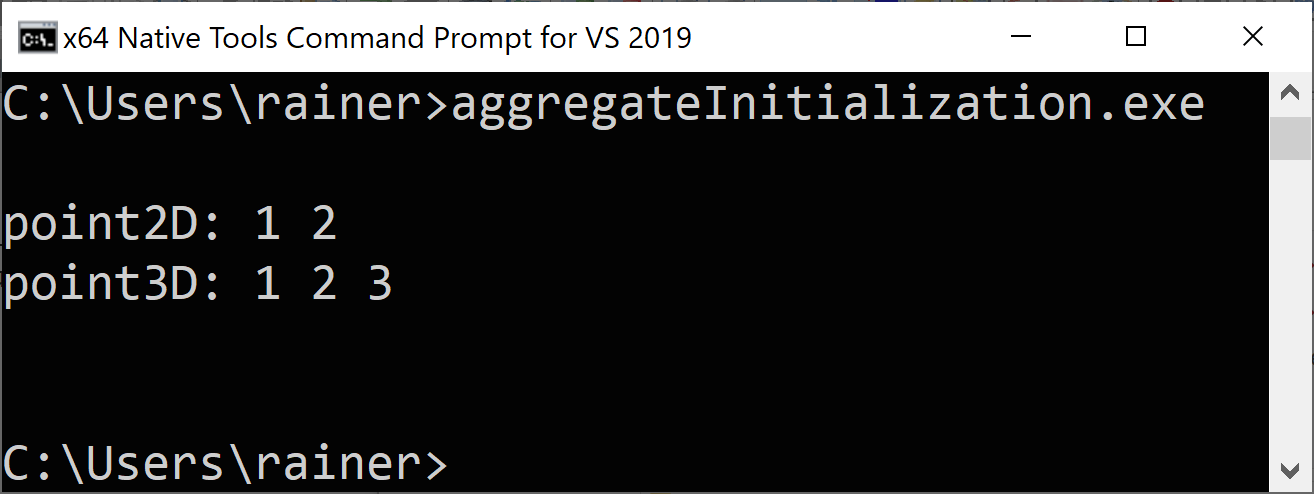
\includegraphics[width=1.0\textwidth]{content/2/chapter3/images/5.png}\\
Aggregate initialization
\end{center}

The aggregate initialization is quite error-prone, because you can swap the constructor arguments, and you will never notice. Explicit is better than implicit. Let’s see what that means. Take a look at how designated initializers from \href{https://en.wikipedia.org/wiki/C99}{C99}, now part of the C++ standard, kick in.

\noindent
Designated initialization
\begin{lstlisting}[style=styleCXX]
struct Point2D{
	int x;
	int y;
};

class Point3D{
public:
	int x;
	int y;
	int z;
};

int main(){

	Point2D point2D {.x = 1, .y = 2};
	// Point2D point2d {.y = 2, .x = 1}; // error
	Point3D point3D {.x = 1, .y = 2, .z = 2};
	// Point3D point3D {.x = 1, .z = 2} // {1, 0, 2}


	std::cout << "point2D: " << point2D.x << " " << point2D.y << "\n";
	std::cout << "point3D: " << point3D.x << " " << point3D.y << " " << point3D.z
		      << "\n";

}
\end{lstlisting}

The arguments for the instances of Point2 and Point3D are explicitly named. The output of the program is identical to the output of the previous one. The commented-out lines 16 and 18 are quite interesting. Line 16 would give an error because the order of the designators does not match the declaration order of the data members. As for line 18, the designator for y is missing. In this case, y is initialized to 0, such as when using braced initialization list {1, 0, 3}.

\subsubsubsection{3.2.2\hspace{0.2cm}Designated Initialization}

The new consteval specifier, which was added in C++20, creates an immediate function. For an immediate function, every call of the function must produce a compile-time constant expression.
An immediate function is implicitly a constexpr function but not necessarily the other way around.

\noindent
An immediate function
\begin{lstlisting}[style=styleCXX]
consteval int sqr(int n) {
	return n*n;
}
constexpr int r = sqr(100); // OK

int x = 100;
int r2 = sqr(x); // Error
\end{lstlisting}

The final assignment gives an error because x is not a constant expression and, therefore, sqr(x) cannot be performed at compile time 

constinit ensures that the variable with static storage duration or thread storage duration is initialized at compile time. Static storage duration means that the object is allocated when the program begins and is deallocated when the program ends. Thread storage duration means that the objects lifetime is bound to the lifetime of the thread.

constinit ensures for this kind of variable (static storage duration or thread storage duration) that they are initialized at compile time. constinit does not imply constness.

\subsubsubsection{3.2.4\hspace{0.2cm}Template Improvements}

C++20 offers various improvements to programming with templates. A generic constructor is a catch-all constructor because you can invoke it with any type.

\noindent
An implicit and explicit generic constructor
\begin{lstlisting}[style=styleCXX]
struct Implicit {
	template <typename T>
	Implicit(T t) {
		std::cout << t << '\n';
	}
};

struct Explicit {
	template <typename T>
	explicit Explicit(T t) {
		std::cout << t << '\n';
	}
};

Explicit exp1 = "implicit"; // Error
Explicit exp2{"explicit"};
\end{lstlisting}

The generic constructor of the class Implicit is way too generic. By putting the keyword explicit in front of the constructor, as for Explicit, the constructor becomes explicit. This means that implicit conversions are not valid anymore.

\subsubsubsection{3.2.5\hspace{0.2cm}Lambda Improvements}

Lambdas get many improvements in C++20. They can have template parameters, can be used in unevaluated contexts, and stateless lambdas can also be default-constructed and copy-assigned. Furthermore, the compiler can now detect when you implicitly copy the this pointer, which means a significant cause of undefined behavior with lambdas is gone.

If you want to define a lambda that accepts only a std::vector, template parameters for lambdas enable this:

\noindent
Template parameters for lambdas
\begin{lstlisting}[style=styleCXX]
auto foo = []<typename T>(std::vector<T> const& vec) {
		// do vector-specific stuff
	};
\end{lstlisting}

\subsubsubsection{3.2.6\hspace{0.2cm}New Attributes}

C++20 has new attributes, including [[likely]] and [[unlikely]]. Both attributes allow us to give the optimizer a hint, specifying which path of execution is more or less likely.

\noindent
The attribute [[likely]]
\begin{lstlisting}[style=styleCXX]
for(size_t i=0; i < v.size(); ++i){
	if (v[i] < 0) [[likely]] sum -= sqrt(-v[i]);
	else sum += sqrt(v[i]);
}
\end{lstlisting}